\section{Evaluation}

\subsection{Testing Methodology}
In order to evaluate the functionality of the application a series of tests were conducted.
To assure that the results are consisted and comparable, the same setup, prompt, input data was used for each run.
There was also a focus of using the same scenes and objects for each test to make it easier to compare results and find outliers.
The input and some of the results can be found in the appendix.
For classification and segmentation the Gemini Pro 2.5 model that was released on the 16th of June 2025 was used.

Throughout the later development of the application the gemini-2.5-pro-preview-05-06 model was used.
With this configuration we were able to get good results and valid outputs.
Since the release of further versions the quality as decreased significantly.
Especially the segmentation quality and validity of the structured json outputs.
The evaluation is still using the newest model though, since it is the most recent version and therefore a current representation of the apps capabilities.
Additionally, it is not possible to use the older model anymore, since it now redirects to the newest version \cite{googleGemini25Pro2025}. 

\subsection{Tool Usage}
A very important aspect is the correct use of the function calling.
When the live api detects that a user might want a more complex operation, like the distance to a specific object, or more complex navigation instructions, it will call a function that triggers the needed process.
In order to evaluate the tool usage, a series of tests were conducted, where the live api needed to use function calling to conduct an answer.
throughout the tests multiple values for temperature, top k and top p were used to see the effect on the tool usage.
There it was found, that there was no significant impact of these values in situations in which the model was not able to correctly use function calling.
Currently the values are set to temperature 0.1, top k 64 and top p 0.9.
Is seems like regardless of the values used, there are constellations in which the model is not able to function correctly.
A example of this can be seen in the following screenshot \ref{fig:tool_usage}.
It is not possible to directly identify the reason for this, as it is also unclear how the model uses the temperature, top k and top p values.
Though it can be suspected that a better system prompt and a more detailed function description could help in these cases.
Additionally, it is also possible to force function calling which could be tried as a normal conversation at a temperature of 0.1 as currently used is not working anyway.

\begin{figure}[H]
\centering
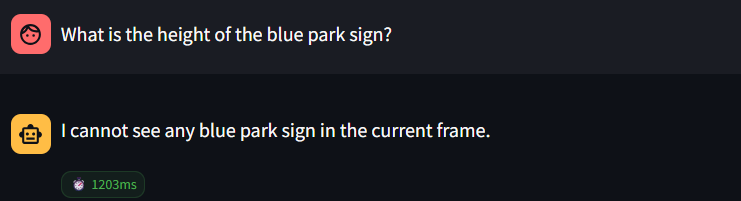
\includegraphics[width=0.4\textwidth]{figures/tool_usage.png}
\caption{Tool usage results for the same scene in multiple runs.}
\Description{A screenshot showing how tool use was not working in a specific run}
\label{fig:tool_usage}
\end{figure}


\subsection{Distance Calculation}

In order to evaluate the distance calculation in relation to the segmentation and a series of tests were conducted using the Gemini Pro model.
Because there is no labelled dataset available for this task it was not possible to create a ground truth for specific objects.
Instead, the distance calculation was evaluated by comparing the results of multiple runs against each other.
This way it is possible to see the run to run variance of the calculation and get a feel for the accuracy and consistency.
In order to create a accurate comparison the same picture, depth map and prompt was used in each run.
All of the runs did a new detection of objects in the scene. 
This way it is also possible to see the variance in object detection.
There it could be seen that a full segmentation of an entire scene reaching the limits of the model, with can result in defect or wrong json outputs.
The results show that objects that are about 4 to 5 meters away from the camera can be detected with consisted distance values \ref{fig:distance_calculation}.
Only on objects that are further away larger errors can be measured.
At this range another issue can also be seen in the lidar sensor which is only rated for about 10 meters on the iPhone 16 Pro \cite{applelidar2025}.

\begin{figure}[H]
\centering
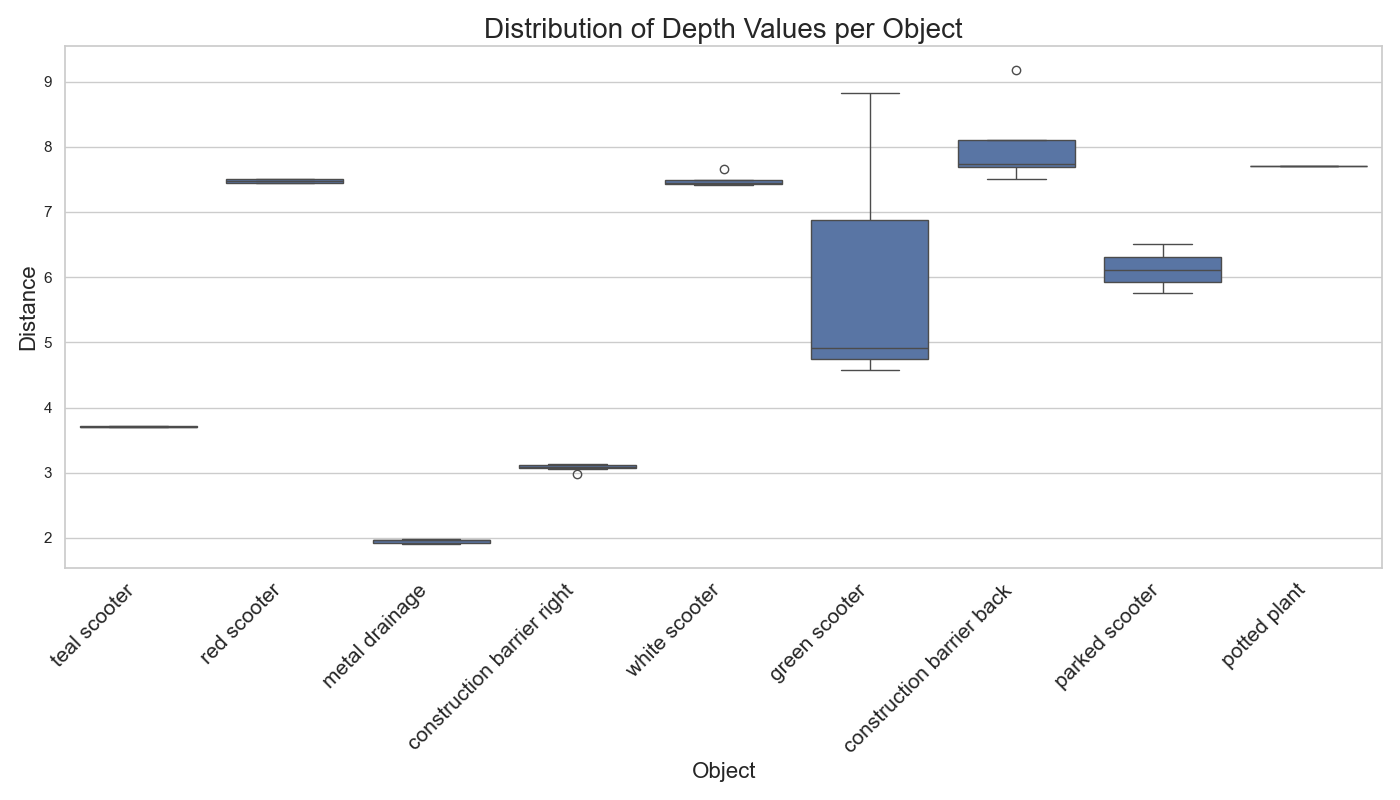
\includegraphics[width=0.4\textwidth]{figures/depth_distribution.png}
\caption{Distance calculation results for the same scene in multiple runs.}
\Description{A chart or graph showing the distribution of distance calculations across multiple test runs for the same scene, illustrating the variance and consistency in depth estimation results.}
\label{fig:distance_calculation}
\end{figure}

\subsection{Segmentation Quality}

Now that we have a visual representation of the average distance we should also take a look at the quality of the segmentation masks that were generated in each run.
The masks were ranked based on the following criteria:
\begin{itemize}
    \item \textbf{Good:} The mask is accurate and covers the object completely.
    \item \textbf{Too big:} The mask is larger than the object, but still covers it.
    \item \textbf{Too little:} The mask is smaller than the object, but still covers a significant part of it.
    \item \textbf{Wrong:} The mask does not cover the object at all or covers the wrong object.
\end{itemize}

As you can see in the Table \ref{tab:segmentation_quality} the segmentation masks vary in quality between different objects but not so much between runs.
For example, the bike was segmented correctly in every run, with one being off by a little bit.
Meanwhile the trash can was not detected at all even though it was clearly visible on screen and could be a potential hazard for the user.
The scooter was always detected in the right position, but the small size of the handlebar made it difficult for the model to segment it correctly.
This is not a problem in this case, since the depth estimation can still work as intended with the segmentation mask not being perfect.
As already mentioned, the tests where conducted on the new Gemini Pro 2.5 model, which could harm quality.

\begin{table}[H]
\centering
\resizebox{\columnwidth}{!}{%
\begin{tabular}{|l|cccc|c|}
\hline
 & \multicolumn{4}{c|}{Segmentation quality} & \\
\cline{2-5}
 & High Fidelity & Oversegmentation & Undersegmentation & Segmentation Failure & Sum of tries \\
\hline
Teal Scooter &2 & 1& 1 & 1 & 5 \\
Trash can & & & & 5 & 5 \\
Bike & 4 & 1 & & & 5 \\
\hline
\end{tabular}%
}
\caption{Segmentation quality of different objects throughout different runs.}
\label{tab:segmentation_quality}
\end{table}